\documentclass[a4paper, 12pt, titlepage]{article}

\usepackage{graphicx, color} %for å inkludere grafikk
\usepackage{verbatim, color} %for å inkludere filer med tegn LaTeX ikke liker. \verbatiminput{verb.txt}
%\usepackage{gensymb} %gensymb Symbols Defined to Work in Both Math and Text Mode 

\usepackage[T1]{fontenc} %for å bruke æøå. upgrades to 256 bit encoding. More characters
\usepackage[utf8]{inputenc} %Kan forandres til latin1. utf8 gir norske tegn
%inputenc allows the user to input accented characters directly from the keyboard;
%fontenc is oriented to output, that is, what fonts to use for printing characters.
%\usepackage[norsk]{babel} 

\usepackage{pdfpages} %Importing external pdf-pages
\usepackage[compact]{titlesec} %Spacing for two-column document

\usepackage{textcomp} % make degrees centigrade symbols, euros, etc
\usepackage{amsmath, amssymb} %e.g. \begin{theorem}[Pythagoras], \begin{proof} or {align}
\usepackage{amsbsy, amsfonts} %\pmb for annerledes boldfont
\usepackage{parskip} %Space between paragraphs
\usepackage{float} %Im­proves the in­ter­face for defin­ing float­ing ob­jects such as fig­ures and ta­bles.
\usepackage{simplewick}
\usepackage{libertine} 
\usepackage{siunitx} % SI units. Example: \SI{100}{\micro\meter}

\usepackage{geometry} % Definerer marger. 
 %\geometry{headhight=1mm}
 \geometry{top=20mm, bottom=20mm, left=30mm, right=30mm} % Marger i mm. Total bredde er 210mm



\author{Wilhelm Holmen}
\title{FYS4411 Project 3}

\begin{document}
 \maketitle
 \newpage

 \section*{Variational Monte-Carlo for the Helium atom}
 The goal of this project is to perform a monte carlo integration to calculate the expectation value of the Hamiltonian, i.e. the expectation value of the ground state energy for the Helium, Beryllium and Neon atom.  
 \begin{align}
 	\left< E \right> = \frac{\int d \mathbf{r_1} d \mathbf{r_2} \psi_T^*(r_1,r_2) \hat H \psi_T(r_1,r_2)}{\int d \mathbf{r_1} d \mathbf{r_2} \psi_T^*(r_1,r_2) \psi_T(r_1,r_2)}
 	\label{ExpectationValue}
 \end{align}
 This will be a many-dimensional integral, and Monte Carlo integration combined with the Metropolis algorith is most efficient for this kind of problem. We define a new quantity, local energy
 \begin{align*}
 	E_L = \frac{\hat H \Psi}{\Psi}
 \end{align*}
 We can reduce the integral in (\ref{ExpectationValue}) to 
 \begin{align}
 	\int E_L d \mathbf{r} 
 \end{align}

 The wavefunction is not known for neither the Helium, Beryllium or Neon atom. Therefore we need to make a guess, and a natural starting point is to use the Hydrogen orbitals. Since both the electrons occupy the 1s-state, a first guess for the helium atom will be a trial wave function will be
 \begin{align*}
 	\Psi_T(r_1,r_2) = e^{-\alpha(r_1 + r_2)}
 \end{align*}

 In the Metropolis algorithm, I will check wether a move given by, $\mathbf{R^{'}} = \mathbf{R} + \delta \cdot r $, will be accepted. $r$ is a random number in $[0,1]$. The acceptance criteria is given by
 \begin{align*}
 	\frac{P(\mathbf{R^{'}} )}{P(\mathbf{R} )} = \frac{\int d \mathbf{R^{'}} \psi^*_T(\mathbf{R^{'}} ) \psi_T(\mathbf{R^{'}} )}{\int d \mathbf{R} \psi^*_T(\mathbf{R}) \psi_T(\mathbf{R} )} \geq r
 \end{align*}

 Because of the variational princible, the trial energy will always be higher than the true energy. Therefore we can adjust $\alpha$ and the steplength $\delta$ until we get the lowest possible energy. The best steplength $\delta$ is a steplength that will accept around $50\%$ of the proposed steps. 

 The first attempt at finding the ground state energy for Helium is found in the code for Project 1. figure (\ref{Helium1}) shows the variance and energy as we vary the parameter alpha. 

 \begin{figure}[H]
 	\centering
 	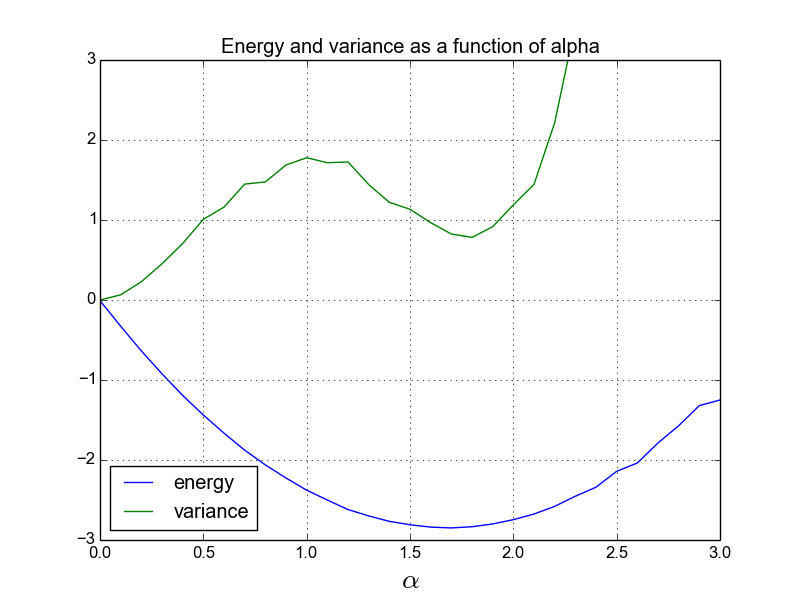
\includegraphics[width=\textwidth]{../python_programs/EnergyVariance_helium1.png}
 	\label{Helium1}
 \end{figure}

 By looking closer at the energy and variance around $\alpha = 1.68$ in figure (\ref{Helium2}), we see that we get an energy of $\left<E\right> = -2.84997$, with a variance of $\sigma ^2 = 0.932912$. This is too far off from the best experimental value of $E_{experimental} = -2.903$. We see however that the variance is smaller for $\alpha = 1.8$, $1.9$ and $1.6$. But by the variational principle, we want as low energy as possible, so we choose the best $\alpha$ as $1.68$. 
 
 \begin{figure}[H]
 	\centering
 	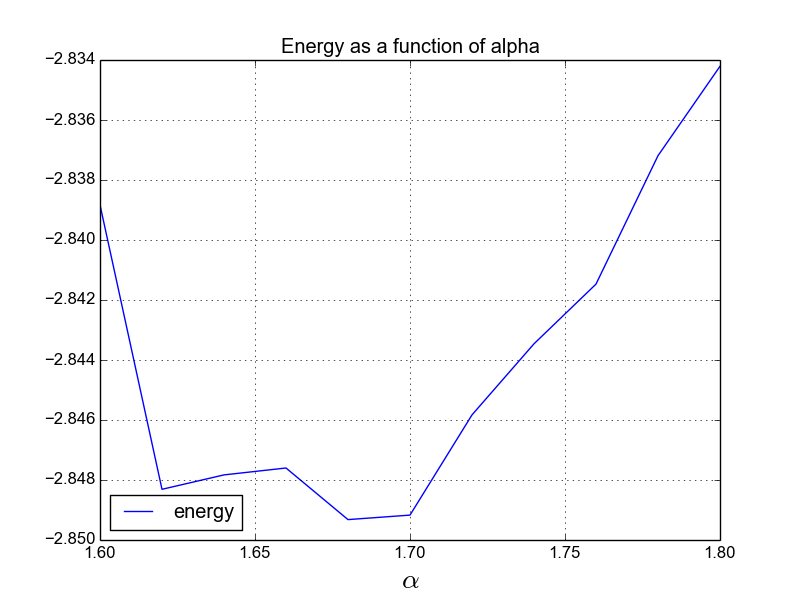
\includegraphics[width=\textwidth]{../python_programs/EnergyVariance_helium2.png}
 	\label{Helium2}
 \end{figure}

 \section*{Jastrow factor}

 We can get a better result by improving our trial wave function, $\Psi_T$. We can introduce a factor known as the Jastrow factor. 
 \begin{align*}
 	\Psi_T(r_1,r_2) = e^{-\alpha(r_1 + r_2)}e^{\frac{r_{12}}{2(1+\beta r_{12})}}
 \end{align*}
 Where $r_{12} = |r_1 - r_2|$. 

 This is a factor that takes the electron repulsion into account. Again, using the code in project one I get the plot in figure (\ref{Helium3}).
 
 By varying $\alpha$ and $\beta$ to find the lowest energy, we see that we can get a lower energy. Namely $E = -2.89207$ for $\alpha = 1.75$ and $\beta = 0.3$. 

 \begin{figure}[H]
 	\centering
 	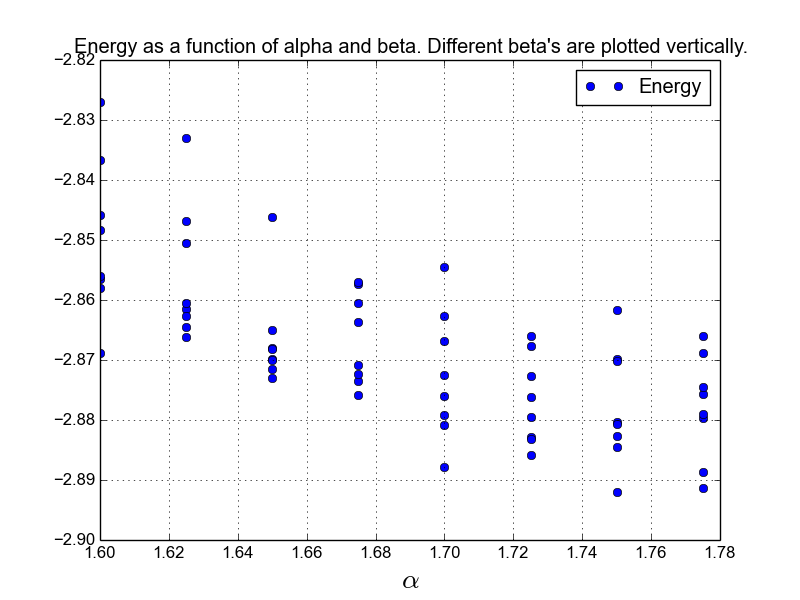
\includegraphics[width=\textwidth]{../python_programs/EnergyVariance_helium5.png}
 	\label{Helium3}
 \end{figure}


 \begin{section}{Analytical calculation of the local energy}
 Calculating the kinetic energy numerically is costly. One can considerably reduce computational time by using a closed form expression for the energy. 

 We have trial wavefunction 
 \begin{align*}
 	\Psi = e^{-\alpha(r_1 + r_2)}
 \end{align*}
 and we want to calculate the local energy given by
 \begin{align*}
 	E_L = \frac{1}{\Psi} \hat H \Psi
 \end{align*}
 where
 \begin{align*}
 	\hat H = -\frac{\nabla_1^2}{2} - \frac{\nabla_2^2}{2} - \frac{2}{r_1} - \frac{2}{r_2} + \frac{1}{r_{12}}
 \end{align*}
 Rewriting	
 \begin{align*}
 	T_{L1} = \frac{1}{\Psi} \left( -\frac{\nabla_1^2}{2} - \frac{\nabla_2^2}{2} \right) \Psi
 \end{align*}
 \begin{align*}
 	V_{L1} = \frac{1}{\Psi} \left( - \frac{2}{r_1} - \frac{2}{r_2} + \frac{1}{r_{12}} \right) \Psi
 \end{align*}
 Doing the calculations, we find that
 \begin{align*}
 	T_{L1} = -\frac{1}{2} \frac{1}{\Psi} \left( \frac{1}{r_1^2} \frac{\partial}{\partial r_1} \left( r_1^2 \frac{\partial}{\partial r_1} \Psi \right) + \frac{1}{r_2^2} \frac{\partial}{\partial r_2} \left( r_2^2 \frac{\partial}{\partial r_2} \Psi \right) \right)
 \end{align*}
 \begin{align*}
 	T_{L1} = -\frac{1}{2} \left( -\frac{2}{r_1}\alpha + \alpha^2 - \frac{2}{r_2} + \alpha^2 \right)
 \end{align*}
 Adding $T_{L1}$ and $V_{L1}$ 
 \begin{align*}
 	E_{L1} = \left( \alpha - 2 \right) \left( \frac{1}{r_1} + \frac{1}{r_2} \right) + \frac{1}{r_{12}} - \alpha^2 
 \end{align*}

 Introducing the Jastrow factor, one can rewrite the wavefunction
 as a product of the direct term and the corrolation term. 
 \begin{align*}
 	\Psi = \Psi_D \Psi_C
 \end{align*}
 We want to calculate the kinetic energy and divide by the wavefunction.
 \begin{align*}
 	T_{L2} = \frac{1}{\Psi} \frac{-\nabla^2}{2} \Psi
 \end{align*}
 Using the chain rule. This equation must be calculated for both particles. 
 \begin{align}
 	T_{L2} = -\frac{1}{2} \left( \frac{1}{\Psi_D}\nabla^2 \Psi_D + 2 \frac{1}{\Psi_D \Psi_C} \nabla \Psi_D \cdot \nabla \Psi_C + \nabla^2 \Psi_C \right)
 	\label{T_L2}
 \end{align}
 The first term is easily calculated, as it is the same as for $E_{L1}$
 \begin{align*}
 	\frac{1}{\Psi_D}\nabla^2 \Psi_D =  -\frac{2}{r_1}\alpha + \alpha^2 
 \end{align*}

 Calculating the second term
 \begin{align*}
 	\frac{1}{\Psi_D} \nabla \Psi_D = \frac{1}{\Psi_D} \frac{\partial}{\partial r} \Psi_D \hat e_r 
 \end{align*}
 \begin{align}
 	\frac{1}{\Psi_D} \nabla \Psi_D = -\alpha \hat e_r
 \end{align}
 When differentiating the corrolation term, given by
 \begin{align*}
 	e^{\frac{r_{12}}{2\left(1 + \beta r_{12} \right)}}
 \end{align*}
 One must use that
 \begin{align}
 	\frac{\partial}{\partial r_i} r_{12} = (-1)^{i+1} \frac{\vec r_1 - \vec r_2}{r_{12}} \hat e_{ri}
 \end{align}

 \begin{align*}
 	\frac{1}{\Psi_C} \nabla \Psi_C = \frac{1}{\Psi_C} \frac{\partial}{\partial r} \Psi_C \hat e_r 
 \end{align*}
 Giving for particle, $i$
 \begin{align*}
 	\frac{1}{\Psi_C} \nabla \Psi_C = (-1)^{i+1} \frac{\vec r_1 - \vec r_2}{2r_{12} \left(1+\beta r_{12} \right)}
 \end{align*}
 Finally multiplying and adding both particles. 
 \begin{align}
 	\frac{\nabla_1 \Psi_D}{\Psi_D} \cdot \frac{\nabla_1 \Psi_C }{\Psi_C} + \frac{\nabla_2 \Psi_D}{\Psi_D}  \cdot \frac{\nabla_2 \Psi_C}{\Psi_C}  = \frac{-1}{\left(1+\beta r_{12} \right)} \left( \frac{\alpha(r_1 + r_2)}{r_{12}} \left(1 - \frac{\vec r_1 \cdot \vec r_2)}{r_1 r_2} \right)  \right)
 \end{align} 

 Now, to calculate the last term in (\ref{T_L2}). 
 \begin{align}
 	\frac{\nabla^2 \Psi_C}{\Psi_C} = \frac{1}{\Psi_C} \left( \frac{2}{r} \frac{\partial}{\partial r}\Psi_C + \frac{\partial^2 }{\partial r^2} \Psi_C \right)
 \end{align}
 Looking at the first part for both particles
 \begin{align*}
 	\frac{2}{r_1} \frac{\vec r_1 - \vec r_2}{2r_{12} \left(1+\beta r_{12} \right)} \frac{\vec r_1}{r_1} + \frac{2}{r_1} \frac{\vec r_2 - \vec r_1}{2r_{12} \left(1+\beta r_{12} \right)} \frac{\vec r_2}{r_2}
 \end{align*}
 Sorting this gives
 \begin{align*}
 	\frac{2}{r_{12}(1+\beta r_{12})^2} - \frac{\vec r_1 \cdot \vec r_2}{r_{12} r_1^2 (1 +\beta r_{12})^2} - \frac{\vec r_1 \cdot \vec r_2}{r_{12} r_2^2 (1+\beta r_{12})^2}
 \end{align*}
 The second part for particle 1
 \begin{align*}
 	\frac{1}{\Psi_C} \frac{\partial^2 }{\partial r^2} \Psi_C = \left( \frac{\vec r_1 - \vec r_2}{2r_{12} \left(1+\beta r_{12} \right)} \hat e_{r1} \right)^2 + \frac{\partial}{\partial r_1} \left( \frac{\vec r_1 - \vec r_2}{2r_{12} \left(1+\beta r_{12}  \right)} \hat e_{r1} \right) 
 \end{align*}
 \begin{align*}
 	\frac{1}{4(1+\beta r_{12})^4} + \frac{\beta}{(1+\beta r_{12})^3}
 \end{align*}
 Combining these calculations
 \begin{align*}
 	 \frac{\nabla^2 \Psi_C}{\Psi_C} = \frac{1}{r_{12}(1+\beta r_{12})^2} + \frac{1}{4(1+\beta r_{12})^4} - \frac{\beta}{(1+\beta r_{12})^3}
 \end{align*}
 Combining, we get the $T_{L2}$
 
 Giving the total local energy
 \begin{align*}
 	E_{L2} = E_{L1} + \frac{1}{2(1+\beta r_{12})^2} \left[ \frac{\alpha (r1+r2)}{r_{12}} \left(1 - \frac{\vec r_1 \cdot \vec r_2}{r_1 r_2} \right) - \frac{1}{2(1+\beta r_{12})^2} - \frac{2}{r_{12}} + \frac{2 \beta}{1 + \beta r_{12}} \right]
 \end{align*}

 More general expressions are used in the code in Project 3. 
 \end{section}

\section*{Importance Sampling}
 Up until now we have used a brute force Metropolis algorithm with a fixed step length. I will now introduce Importance sampling, which takes the force acting on the particle into account.
 \begin{align*}
 	\mathbf{F} = 2 \frac{1}{\Psi_T} \nabla \Psi_T	
 \end{align*}
 This foce can be calculated both numerically and analytically, where the analytical calculation is much faster. However, the analytical calculation does not give satisfactory results on atoms larger than Helium in my code, so I will use numerical differentiation when calculating on Beryllium and Neon. 

 We can see from the plot below that using $dt = 10^-3$, we get stable results. A smaller $dt$ probably gives rise to different kinds of errors, like truncation errors etc. Using this dt, we get $-2.86462$ as the energy using code from Project1 with numerical differentiation. 
 \begin{figure}[H] 
 	\centering
 	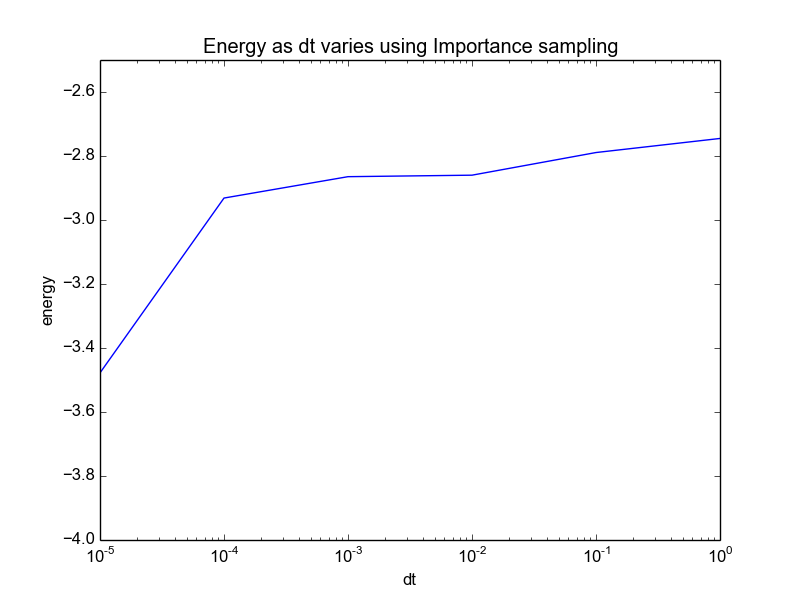
\includegraphics[width=\textwidth]{../python_programs/ImportanceSampling_Helium_dt.png}
 \end{figure}

\section*{Statistical Analysis}
 A Monte Carlo simulation gives rise to two kinds of error. Systematic errors and statistical errors. Systematic errors are due to limitations of the applied models and faulty implementations. Here I will explore methods to estimate the statistical error. 

 Given a set of local energies, the variance is a measure of the spread from the true mean. The definition is
 \begin{align*}
 	\text{Var}(E) = \left< E^2 \right> - \left< E \right> ^2 
 \end{align*}
 Unfortunatly we do not know the true mean in a Monte-Carlo simulation. The computed average $\overline E$ is an approximation to the exact mean, and we do the following approximation
 \begin{align*}
 	\text{Var}(E) \approx \overline{E^2} - \overline{E}^2 
 \end{align*}
 For the case where we have the exact wave function, the variance becomes $0$, so the variance is an excellent measure of how close we are to the exact wave function. The variance however is \textit{not} a direct measure of the error. The standard deviation, the square root of the variance is related of the \textit{spread} in the sampled value. 
 \begin{align}
 	\sigma ^2(x) = \text{Var}(x)
 	\label{deviation}
 \end{align}
 This does not account for the samples being corrolated. Two samples, $x$ and $y$ are corrolated if the \textit{Covariance} is non-zero.
 \begin{align*}
 	\text{Cov}(x,y) = \left< xy \right> - \left< x \right> \left<y \right> 
 \end{align*}
 The diagonal elements of the Covariance is the Variance. By ignoring the corrolations, one get an error estimate that is generally too small. Given the true deviation, $\sigma_e$ and $\sigma$ from (\ref{deviation}) we have
 \begin{align*}
 	\sigma_c \geq \sigma
 \end{align*}

 The most interesting quantity when doing statistical analysis is not the error of single samples. It is the error of the mean value. One can show that the variance for the mean value, $m$ is 
 \begin{align}
 	\sigma^2 (m) = \frac{1}{n} \text{Cov}(x)
 	\label{covariance}
 \end{align}
 Where n is the number of samples used to calculate $m$ and 
 \begin{align*}
 	m = \frac{1}{n} \sum_i^n x_i
 \end{align*}
 Calculating the Covariance is an expensive process for a large sample set, so we need a better way to calculate this. 

\section*{Blocking}
 There is no need to do statistical analysis within the Monte-Carlo simulation. By storing the data set, one can estimate the error post process. An efficient algorithm for this is called blocking. 

 Given a set of $N$ samples from a single Monte-Carlo process. This set is divided into $n$ blocks of size $n_b = N/n$. Now we can treat each block as an individual simulation to calculate the variance of a calculated mean, $m$. This will in turn give us the covariance by (\ref{covariance}).
 \begin{align*}
 	\sigma^2 (m) = \left<m^2\right> - \left<m\right>^2 
 \end{align*}

 One can not know beforehand which block size is optimal to compute the exact error. One can, however, plot the variance against different block sizes. The curve should be stable over a span of block sizes. This plateau will serve as a reasonable approximation to the covariance. 

\section*{One-body density}
 The one-body density is defined as
 \begin{align*}
 	\rho(r_1) = \int_{r_2} .. \int_{r_N} | \Phi(r_1 r_2 .. r_N) |^2 dr_2 .. dr_N
 \end{align*}

 The distribution $|\Phi(r)|^2$ describes the distribution of a particle in the system. The one-body density $\rho(r_1)$ describes the simultaneous distribution of every particle in the system. $\rho(r_1) dr_1 $ represents the probability of finding \textit{any} particle in the volume element $dr_1$ as oppsed to $|\Phi(r)|^2$ giving the probability of finding \textit{particle $r_1$} in the volume element $dr_1$. Due to the indistinguishable nature of the particles, any of the coordinates contain information about all the particles. I will therefore normalize this density to the number of particles $N$ and not $1$ which is common for the one-particle density. 

 The way this is computed in a Monte Carlo simulation is by taking snapshots of all positions for every timestep, then constructing a histogram to construct an approximation to the wave function.

 The charge density for a single particle is given by 
 \begin{align*}
 	\rho_q (r) = q |\Psi(r)|^2
 \end{align*}
 However, since we already have computed the many-body probability density, we can use this instead to get the many-body charge density of the system. 
 \begin{align*}
 	\rho_q (r) = Q \rho(r_1)
 \end{align*}

\section*{Generalizing wavefunction using Slater determinants}
 Up until now, I have been operating with the trial WaveFunction $\Psi_D = e^{-\alpha(r_1 + r_2)}$. One can write a many-particle wavefunction as a Slater determinant. This way of writing is consistent with Pauli's principle. The determinant consists of single particle wave functions. In this project, the wave functions used are the hydrogen orbitals. 

 \begin{align*}
 	\Psi_D = \frac{1}{\sqrt{(N!)}}\left| \begin{matrix}
 		\psi_1(r_1) & \psi_1(r_2) & ... & \psi_1(r_N) \\
 		\psi_2(r_1) & \psi_2(r_2) & ... & \psi_2(r_N) \\
 		... & & & ... \\
 		\psi_N(r_1) & \psi_N(r_2) & ... & \psi_N(r_N) 
 	\end{matrix} \right|
 \end{align*}

 Since we are looking at rations between wavefunctions, the factor in front does not matter. However the inverse of this matrix is zero, because the one-particle wavefunctions are equal for opposite spins. $\psi_{1s \uparrow}(r_1) = \psi_{1s\downarrow}(r_1)$. Because the Hamiltonian is spin-independent, we can factorize the determinant by writing the determinant as a product of a spin-up determinant and a spin-down determinant. The spin up determinant will consist of the firstt half of particles in up-spin states, the spin down will consist of the second half in down-spin states. For Beryllium, this will give

 \begin{align*}
 	\Psi_D = \frac{1}{\sqrt{(N!)}}\left| \begin{matrix}
 		\psi_1(r_1) & \psi_1(r_2) \\
 		\psi_3(r_1) & \psi_3(r_2) \end{matrix} \right| \left| \begin{matrix} \psi_2(r_3) & \psi_2(r_4) \\ \psi_4(r_3) & \psi_4(r_4)
 	\end{matrix} \right|
 \end{align*}

 The program code in Project3 uses this approach for both Helium, Beryllium and Neon. 

\section*{Steepest descent}
 Up until now, I have used measurment by eye to find the optimal values for $\alpha$ and $\beta$. This can be done in a more precise way, namely using methods like steepest descent or Conjugate Gradient method. I have included the steepest descent method in my project.
 If a function $F(x)$ is differentiable and in the neighborhood of a point $\mathbf{a}$, then the function $F(x)$ decreases fastest in the direction of the negative gradient, $-\nabla F(x)$. i.e. we are approaching a minima. Since the variational principle holds for $\left<\hat H\right> $, the best values for $\alpha$ and $\beta$ are the ones giving this minima. 
 \begin{align*}
 	\mathbf{b} = \mathbf{a} - \gamma \nabla F(\mathbf{a}) 
 \end{align*}
 if $\gamma$ is small enough, $F(\mathbf{b}) \leq F(\mathbf{a})$. We can therefore set up the scheme
 \begin{align*}
 	x_{n+1} = x_n - \gamma \nabla F(x_n)
 \end{align*}
 and continue until
 \begin{align*}
 	x_{n+1} - x_n \leq \text{precision}
 \end{align*}

\section*{Final variational Monte-Carlo on Helium}
 By excluding the Jastrow factor and the two-body potential in the local energy, one can test wether the Slater determinant is set up right. By setting $\alpha$ equal to the number of particles, one should get $\left< \hat H \right> = -4$. This can be reproduced, both with the analytical local energy, the numerical local energy, the numerical quantum force and the analytical quantum force. After doing these naive simulations, I include the Jastrow factor and the two-body potential. 

 I have found the optimal parametres for calculating on Helium. I set $\alpha = 1.75$, $\beta = 0.3$, $\text{step} = 1.5$. These results are obtained using the code in Project1. This computation gave an energy of
 \begin{align*}
 	E = -2.89207
 \end{align*}
 Which is pretty close to the best value $-2.903$. 

 A plot of the probability density:
 \begin{figure}[H] 
 	\centering
 	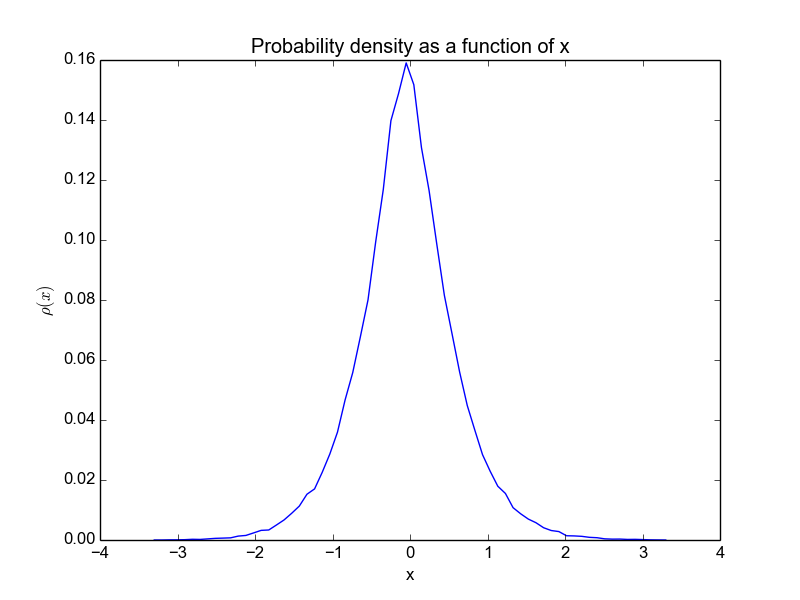
\includegraphics[width=\textwidth]{../python_programs/ProbabilityDensity.png}
 \end{figure}
 Since we only have the 1s-states, the density should be close in shape to the 1s-shape. This density will be more spread out when one take the electron-electron repulsion into account, because the repulsion can be seen as a reduction in the core's charge. 

 By using the blocking analysis, the following plot shows how variance of the mean $E$-value changes when the block size changes. The y-axis shows the total error in the calculation. 
 One see that the error is estimated to be around $0.29$. The spread seams to be pretty uniform and I conclude that the corrolation is low. 
 \begin{figure}[H] 
 	\centering
 	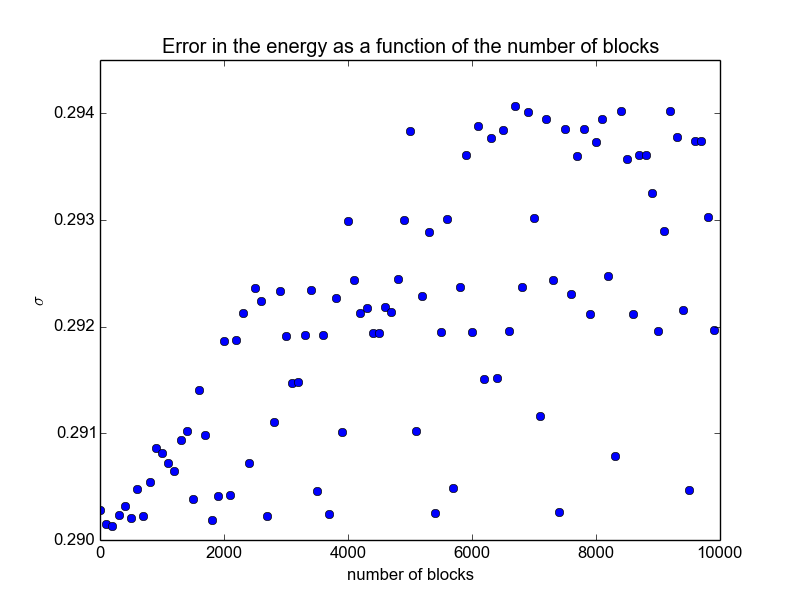
\includegraphics[width=\textwidth]{../python_programs/HeliumBlocking.png}
 \end{figure}

 A short computation time comparison between the numerical and analytical gradients and Laplacians are found in the files, \textit{Helium\_CompareTime.txt}, \textit{Helium\_CompareTime\_ELnum.txt} and \textit{Helium\_CompareTime\_QFnum.txt}. All of them are done with Importance Sampling. 

 We see that the results are about the same, but the time needed for the computation is $33$s for analytical, $52,3$s for the numerical local energy and finally $65.4$s for the numerical quantum force. 

 For the final run on Helium with importance sampling and Steepest descent method, I set $\alpha = 1.75$ as I have seen that this alpha gave the lowest energy when the Jastrow factor was included. The steepest descent method stabilized at $\beta = 0.515163$. I used $10^7$ iterations for each core, so a total of $4 \cdot 10^7$ iterations in the calculation. This running is done with the Importance sampling method, so the only variational parameter that is not perfectly optimized is the value for $\alpha$. This can be fixed by including the Gaussian Orbitals which are a result of Hartree-Fock calculations. They do not have a parameter to be varied, and should for that reason give an optimal value. The result from this calculation is found in the file \textit{Helium\_final\_calculation.txt}. The result gained was
 \begin{align*}
 	E = -2.88538
 \end{align*}

\section*{Variational Monte Carlo on Beryllium}
 Using the code in project 3 to do calculations on Beryllium. First I search for a good value of $\alpha$, looping through 20 different $\alpha$'s from 3 to 4.
 \begin{figure}
 	\centering
 	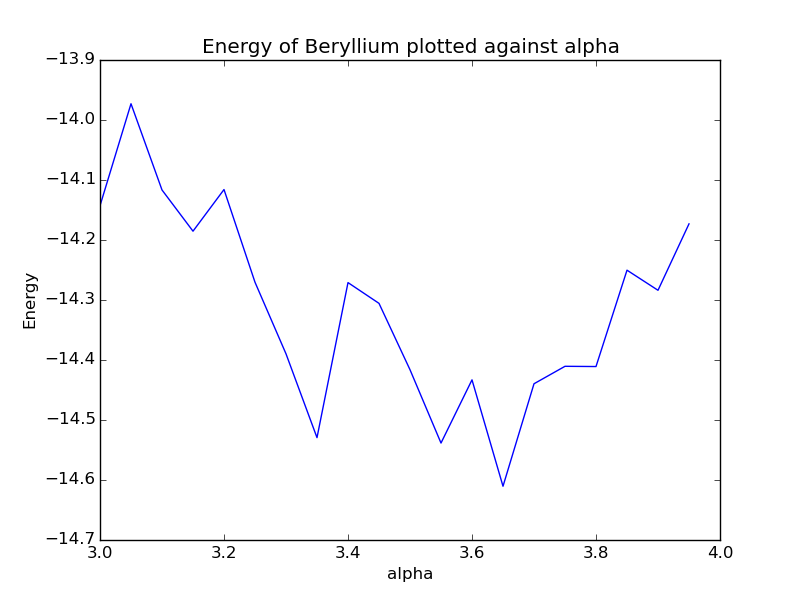
\includegraphics[width=\textwidth]{../python_programs/FindOptimalAlphaBeryllium.png}
 \end{figure}
 As seen in the figure, setting $\alpha = 3.65$ gives the lowest energy. A monte carlo integration with that alpha gives 
 \begin{align*}
 	E = -14.4144
 \end{align*}
 with $10^6$ iterations per core. The result is in the file \textit{Beryllium\_MC.txt}. Following is the one-body density ploted along with a blocking analysis show that the error lies around $3.7$. 
 \begin{figure}
 	\centering
 	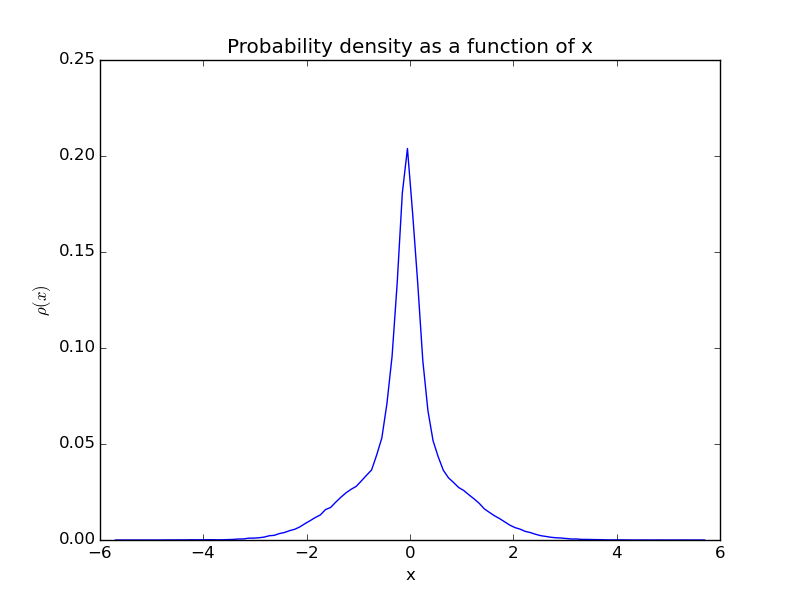
\includegraphics[width=\textwidth]{../python_programs/ProbabilityDensityBeryllium.png}
 	\caption{A plot showing the one-body density in the x-direction for a particle in the Beryllium atom}
 \end{figure}
 \begin{figure}
 	\centering
 	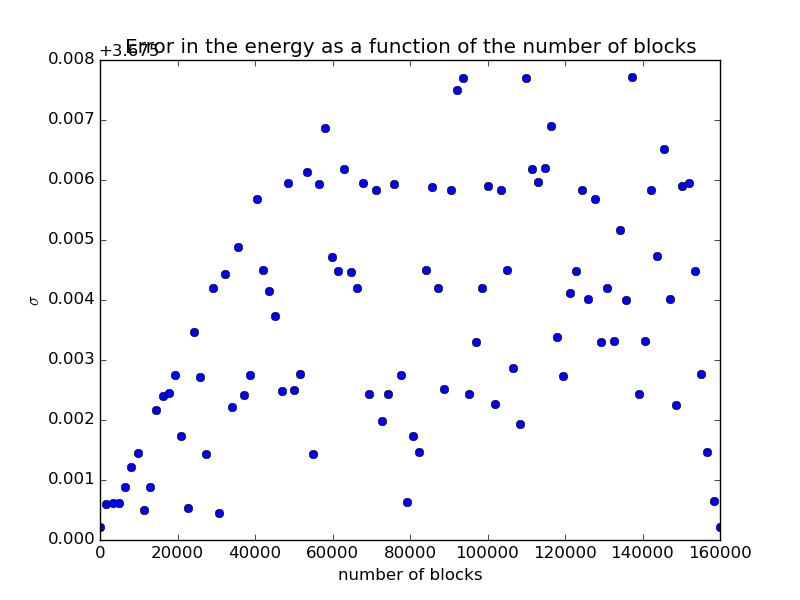
\includegraphics[width=\textwidth]{../python_programs/BerylliumBlocking.png}
 \end{figure}


 Unfortunatly the analytical computation of the quantum force does not give a satisfactory result when increasing particles above $2$, so the run with importance sampling is done with numerical differentiation. I did however not get as low energy with importance sampling as with the brute force Metropolis algorithm. The resulting energy for this computation was $E = -14.0801$. I plotted the one-body density for the brute force algorithm instead, because of a better calculation. The results from this calculation is found in \textit{Beryllium\_IS.txt}. 

 Running without the Jastrow factor, I surprisingly got a result close to the calculation with the factor. The energy was $E = -14.3423$. This is with the potential energy due to the repulsion between the electrons. Removing this repulsion, I get $E = -20$, which is expected. The results are found in \textit{Beryllium\_withoutJastrow.txt} and \textit{Beryllium\_withoutJastrow2.txt}. 
 


 \end{document}